%
% File acl2020.tex
%
%% Based on the style files for ACL 2020, which were
%% Based on the style files for ACL 2018, NAACL 2018/19, which were
%% Based on the style files for ACL-2015, with some improvements
%%  taken from the NAACL-2016 style
%% Based on the style files for ACL-2014, which were, in turn,
%% based on ACL-2013, ACL-2012, ACL-2011, ACL-2010, ACL-IJCNLP-2009,
%% EACL-2009, IJCNLP-2008...
%% Based on the style files for EACL 2006 by 
%%e.agirre@ehu.es or Sergi.Balari@uab.es
%% and that of ACL 08 by Joakim Nivre and Noah Smith

\documentclass[11pt,a4paper]{article}
\usepackage[hyperref]{acl2020}
\usepackage{booktabs}
\usepackage{graphicx}
\usepackage{times}
\usepackage{latexsym}
\renewcommand{\UrlFont}{\ttfamily\small}
\hypersetup{
    colorlinks=true,
    linkcolor=blue,
    filecolor=magenta,      
    urlcolor=blue,
    pdftitle={Representation Engineering via Control Vectors},
    pdfpagemode=FullScreen,
    }


\usepackage{microtype}

\aclfinalcopy % Uncomment this line for the final submission


\newcommand\BibTeX{B\textsc{ib}\TeX}

\title{Representation Engineering via Control Vectors}

\author{Hayden Outlaw \\
  Tulane University / New Orleans, LA \\
  \texttt{houtlaw@tulane.edu} \\\And
  Joe Wagner \\
  Tulane University / New Orleans, LA \\
  \texttt{jwagner3@tulane.edu} \\}

\date{}

\begin{document}
\maketitle
\begin{abstract}
We present an expanded implementation of control vector engineering for the \emph{Mistral-7B-Instruct-v0.1}, in which we pre-compute vector representations of 50 different model behaviors, which we can then enforce in future queries through the addition of the vector to the activation function between each layer. We also add a novel visual representation framework for these control vectors, in terms of their individual weights as well as their magnitude of effect at each layer, and a front-end that allows for implementation of linear combinations of control vectors to induce a mixture of behaviors from the model at a variety of magnitudes. 
\end{abstract}

%

%Title, Author(s) [done]
%Abstract: It should not be more than 300 words. What did you do and what was the main conclusion? [done]
%Introduction: Describe the problem precisely and why it is important.
%Background/Related Work: Summarize at least five related research papers related to your project. How is your project similar/different?
%Approach: What method or algorithm are you using. Are you using an existing library to do so? Did you introduce any new variations to these methods? This section details the framework of your project. Be specific, which means you might want to include equations, figures, plots, etc
%Experiment: What kind of experiments did you do; what kind of dataset(s) you're using; what baseline method are you comparing against; and how you will evaluate your results. Report the results of your experiments in detail, including both quantitative evaluations (show numbers, figures, tables, etc) as well as qualitative evaluations (show images, example results, example errors, etc). Be sure to conduct some "stress testing" of your system using your demo interface. What type of errors does it make and why? Are there any systemic biases you notice in the system (e.g., that would affect one source of data more than others)?
%Conclusion: What have you learned? Suggest future ideas.
%References: list of references cited in your report.
%Screenshots: Include screenshots of your web interface showing a demonstration of your project.









\section{Introduction}
With the recent rise in popularity of language models, steering their behavior either towards desired behavior, or away from undesirable behavior has been critical to ensure that outputs remain in line with what users want, both from explicit information within the query, but also implicitly through the desire to receive a response that mimics certain attributes or adjective such as "helpfulness", "conciseness", "politeness", and "simplicity". The vehicle for inducing these behaviors has long been "prompt engineering", which is the practice of adding instructions implicitly before or after the user's query to overtly "tell" the model what kind of response to return. However, this makes no actual edits to the model's internal weights, can be of limited effectiveness when there are a large number of desired attributes simultaneously, and is vulnerable to malicious further prompt engineering on the part of the user. 

Given a list of known true and false statements, we can use contrastive prompts to extract representations of our desired behavior from the weights within the model. These are called 'control vectors' - and with them, we can manipulate the weights directly within the model, instead of simply adding to the prompt beforehand. With these implicit modifications, not only can we adjust the magnitude of the effect by adjusting the weights within the control vectors, but we can enforce the behavior in a much more robust way that is simultaneously much more effective, and less vulnerable to outside modification from prompt injections or modifications.

\section{Background}
We utilize significant results from the five following projects:

\begin{enumerate}


\item \emph{Representation Engineering: A Top-Down Approach to AI Transparency} ~\cite{zou2023representation}

Zou et al's paper on representation engineering formalizes current progress in the field by prioritizing representations of higher-level concepts above neurons or activation functions for framing models. They introduce the concept of control vectors in order to extract these high-level representations of networks. The utility of control vectors is demonstrated for model analysis and AI transparency. They create control vectors using contrastive prompting and principal component analysis, which are then added onto the activation functions to enforce behaviors, similar to our work. Whereas they focus on model interpretability 



\item \emph{Towards Monosemanticity: Decomposing Language Models with Dictionary Learning} ~\cite{bricken2023towards}

Bricken et al., examine language model interpretability through the lens of monosemanticity and polysemanticity - the study of how one individual neuron or unit can encode information for one or multiple embeddings as a component of a combination of other neurons. They use a sparse autoencoder to generate learned features, as opposed to principal component analysis, which is a more involved process that leans on a greater amount of prior work - however, they had relative success in using these models to extract a high proportion of monosemantic features, and in a way that was relatively model architecture agnostic.

\item \emph{Activation addition: Steering language models without Optimization}~\cite{turner2023activation}

Turner et al do not lean on the concept of 'representation' as much, but do propose the framework of modifying activation functions to steer or control model outputs, specifically by using contrasting prompt pairs to learn a vector, which is then injected into the activation function when multiplied by some parameter scalar.  This paper predominantly focuses on sentiment steering and improving model performance, but is much less concerned with safety, adversarial querying, and jailbreaking than Zou et al.,

\item \emph{A Tutorial on Network Embeddings}~\cite{chen2018network}

Chen et al offer an overview of different ways to extract representation embeddings from models beyond PCA. This is different than the high-level concepts we are trying to learn with control vectors, and rather focuses on the applications of low-dimensional latent node representation. Some of the methods covered include isomaps and local linear embeddings. While somewhat out of the scope of our project, the unsupervised methods are potential strategies we will explore to improve our model.

\item \emph{Representation Engineering Mistral-7B an Acid Trip}~\cite{vogel2024repeng}

Extends and explains the functionality of the repeng python library, which allows for easy use of control vectors with pytorch. Looks beyond the high level representation side of RepE and instead compares it to current methods including prompt engineering and fine tuning. Packaged code provided allows for generating control vectors from contrastive prompts. Whereas Vogel focuses on a wide range of applications for control vectors, our project instead hones in on giving users a variety of trained control vectors which all elicit unique responses. 

\end{enumerate}


\section{Approach}
While these projects include proof of concept, given the high computational cost associated with generating these control vectors, there does not yet exist a user-facing accessible and interpretable mechanism for individuals to implement these control vector schemes. Our approach will focus on using control vectors for further representation engineering and explainability, and as a lens with which to examine the biases and behaviors within foundation models. 

As such, our project has essentially two components - the pre-calculation of conceptual representations within the model, and the frontend component that will pass queries through an evaluation pipeline.

\subsection{Model Architecture}
Since we require manual adjustment of the activation functions between layers, we need an open-source model that is completely accessible at the weight level, while still being relatively lightweight enough to query within a reasonable time for a web application. Much of the relevant literature for this reason utilizes the \emph{Mistral-7B-Instruct-v0.1} \cite{jiang2023mistral} model, which is what we will use as well; while it is a "mixture-of-experts" model and a bit outside of the scope of this course, it includes specific \emph{[INST]} tokens for instructional control which increase the effectiveness of the extraction and control process. We can access the model from \emph{HuggingFace}\footnote{https://huggingface.co/mistralai/Mistral-7B-v0.1} and load it directly into PyTorch with simple license acceptance.

For computational tasks, we use a PC equipped with an NVIDIA 3090 graphical processor -- while it is possible to complete model passes with fewer computational resources, the time required to do so was prohibitive to development and application responsiveness. We note that since this model is pre-trained, all we require are multiple repeated passes from the model as it is, and we do not actually train or otherwise adjust its weights.

\subsection{Control Vector Calculation}
For the calculation of control vectors, we utilize the \emph{Repeng} library \cite{vogel2024repeng}, which builds upon the framework from \cite{zou2023representation}. The calculation process essentially is as follows:
\begin{enumerate}
    \item Identify a desired behavior, or set of behaviors, with a set of corresponding antonyms. e.g., [Joking, Serious], [Drunk, Sober], [Angry, Peaceful], etc.,
    \item Using a cached list of prompts and the Mistral instructional tokens, create a list of contrasting prompt pairs. e.g., "[INST] Act extremely Drunk. [/INST] I am", [INST] Act extremely Sober. [/INST] I am", \dots 
    \item Evaluate the model multiple times across each of the contrasting prompts. At the final layer of the model, collect the hidden state representations. 
    \item With these sets of hidden state representations, take the difference between the positive and negative iterations.
    \item Use a feature extraction method on the relative differences of hidden states to generate a control vector for each layer of the model. In this iteration, we also use single-component principal component analysis.
\end{enumerate}

Again, while this requires multiple passes through the model, no weights are ever adjusted. Also note that a control 'vector' is a list of vectors, with each entry corresponding to one layer for the language model, and each vector within is the same size as the hidden state within each layer individually.

\subsection{Evaluation with Enforced Behavior}
Once the control vectors are calculated, forward passes of the model can be computed with the behavior enforced. To do so, we utilize the \emph{Repeng} ControlModule object, which extends Pytorch Module objects for custom activation function definition. 

In each forward pass, for each layer, the activation function is modified given a normalization flag, a defined operation to combine the control vector into the activation function, and a scalar value. We first check each entry of the hidden state, and create a binary vector that encodes if an entry is nonzero. We then multiply the control vector by this mask - as if an entry is zero in the original layer, it should remain zero after modification. We then potentially normalize the control vector if desired, and multiply it by our chosen scalar multiple. This scalar parameter affects the magnitude of the behavior enforcement. We then combine the original activation function output with the control vector using the chosen operation, and potentially normalize this output as well if desired.


\subsection{Web App}
Our web app in Flask provides users with the ability to select a pre-cached control vector, magnitude of effect, and then to pass a query through the model with their desired control behavior enforced. The app loads the model once locally, and then loads the desired control vector into memory. The user's query is then formatted, passed through the model, and the output is sent back to the frontend to be read. The frontend will also pass the query through the model twice with no control vector loaded (equivalent to a selected magnitude of 0), for comparison and examination of effect. For more information, refer to Appendix \ref{appendix:A}. We note that this requires similarly capable local computation resources - the host has to be able to at least evaluate a local forward pass of the model, which often requires an external GPU processor. Alternatives include web deployment with the inclusion of cloud resources to load and evaluate the model. For implementation, deployment, and source code, see \href{https://github.com/tulane-cmps6730/project-control}{project-control} on Github.


\section{Experiments}

\subsection{Experimental Overview}
In our experiments, we tested the efficacy of control vectors in steering the behavior of the Mistral-7B-Instruct-v0.1 language model without modifying its underlying architecture or training procedures. We aim to demonstrate that control vectors can enforce specific behaviors more effectively and robustly compared to traditional prompt engineering techniques. Our Flask web app offers a simple interface for conducting these experiments - we can quickly adjust the desired behavior and magnitude of our chatbot's response. We calculated and cached control vectors for $100$ synonym-antonym pairs, which range from emotional responses, to more traditional model alignment instructions.

\subsection{Dataset}
The Mistral model is trained on a massive collection of text, but since we utilize it in a pre-trained manner the dataset of focus is the contrastive text prompts. Our experiments utilized a diverse set of text prompts designed to evoke specific behaviors including some of the following: arrogant/humble, precise/vague, succinct/rambling. Each behavior is reflected in the form of a control vector that is trained and saved into the project's data folder. The experiments selected different behaviors and magnitudes, then examined their behavior qualitatively. 

%
%Notes:
%- AI safety
%- Move prompt engineering, flow into jailbreak %and AI safety discussion


\subsection{Visualizations}
For visible inspection, we compute two graphical representations for each control vector. Recall that each "Vector" is a list of vectors, with one for each layer. We compute the average value across all individual vectors in the array to get the average magnitude of effect on each layer, as well as the average vector across all layers. For example, with the desired behavior of "Elated" versus the undesired behavior of "Dejected", Figure \ref{fig:elated_effect} depicts the average control vector across all layers of the model, and Figure \ref{fig:elated_mag} depicts the average weight magnitude for each layer. We can see that the control vector is mostly subtractive, with most values between 0 and -0.025, but with the most noticeable effects in layers 10-15.

While it is possible to depict the entire list of vectors as a two-dimensional array, or potentially as a heatmap, we found that most of the values are so small, and the array so large, that any visual insight is generally lost.

\begin{figure}[!ht]
\centering
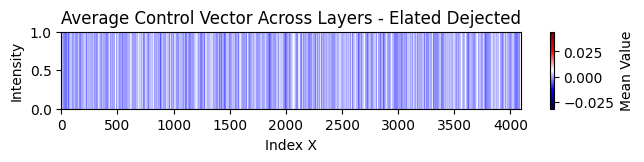
\includegraphics[width = 0.4\textwidth]{assets/Elated_Dejected_mean_values.png}
\caption{Average Control Vector Value across Layers - Elated vs Dejected}
\label{fig:elated_effect}
\end{figure}

\begin{figure}[!ht]
\centering
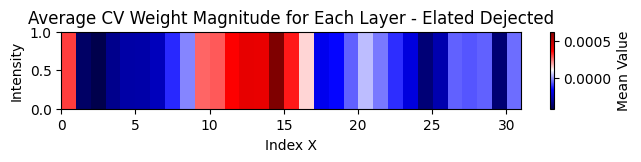
\includegraphics[width = 0.4\textwidth]{assets/Elated_Dejected_mean_values_trans.png}
\caption{Average Control Vector Value for Each Layer - Elated vs Dejected}
\label{fig:elated_mag}
\end{figure}


\subsection{Magnitude of Effect}
When the control vector is added into the activation function, it is first multiplied by a scalar that affects the magnitude of the enforced behavior. Usually, smaller values work better - and while negative values generally correspond to the inverse behavior (or enforcement of the antonym behavior from the training process), the negative values are even more limited in their potential magnitude. Scalars that are too large ruin model outputs, and destroy cogency, as the effect of the control vector eclipses the weights multiplied in each pass. We limit the potential value to be less than $3$ in our application, although the most pronounced effects that are usable seem to be around a value of $2$.

\section{Discussion}
\subsection{Interpretability and Explainability}
The control vector framework presents the capacity to extract and examine potential representations of concepts from within the model, but also the ability to explore the effect that representation has on final output. The visual representations are intuitive, and allow for a more holistic overview of the concept's effects on individual weights, in a way that the effects of prompt engineering would not be possible to capture. 

\subsection{Computation Requirements}
As opposed to fine-tuning, implementing and calculating control vectors is a cheaper and more accessible process. First, the calculation of control vectors is only feature extraction on the results of multiple forward passes - there are no gradients calculated, and no weights adjusted within the model, which greatly reduces the computational cost associated with their generation. Enforcement is also relatively cheap - since a linear function is used to combine the control vector with the hidden weights in each activation function, the cost associated with enforcement is at worst linear with respect to the number of layers in the model. Given that the bulk of the cost is in the vectors' generation, which only needs to be done once, and then can be utilized from a cache with no new learning required, they scale in a useful way for deployment in user-facing utilities such as chatbots.

\subsection{Safety}
Control vectors are also better at controlling model output than prompt engineering in a user-facing manner. Especially given the recent cottage industry that has grown around jailbreaking models towards undesireable behavior using specific adversarial prompts or other injection methods, there is a need for simultaneously transparent and robust control methods. For a given behavior enforced with a control vector ('helpful', 'cautious', 'civil', 'balanced', etc.,) removing the behavior externally using prompt engineering is extremely difficult, as illustrated by Vogel \cite{vogel2024repeng} \footnote{See also: \href{https://vgel.me/posts/representation-engineering/}{Representation Engineering Mistral-7B an Acid Trip}}. However, the other side of this feature is that control vectors provide a very efficient way to jailbreak models that were tuned or aligned to certain behaviors, if the individual layers are accessible. Therefore, for safety purposes, these tools are best suited for scenarios in which developers have direct access to model weights, but users do not - hampering open source accessibility and transparency.

Zou et al., \cite{zou2023representation} also excellently outline the utilization of representation engineering as a tool for transparency with regards to the model itself. While their visualization methods are more advanced than ours, we were aiming for a similar simple visual representation of hidden representations within otherwise intractable layers. Often referred to as 'top-down' research, control vectors also can serve as a useful tool for examining the biases and behaviors of the model itself within its internal representation space. However, we were unable to find useful quantitative insight into the similarities between control vectors and how it translates itno knowledge 

\subsection{Shortcomings}
While this process is generally model-agnostic, in the sense that it is theoretically feasible for any language model with distinct layers and activation functions, as with any representation space the final control vectors are model-specific. For each model architecture, the control vectors have to be calculated from scratch, and do not translate between different model versions or sizes. 

As opposed to prompt engineering, the number of different concepts that can be enforced via control vectors is relatively small. Since the overall magnitude of the changes implemented has to remain below a certain threshold for the responses to remain cogent, implementing multiple different conceptual enforcements required that the magnitudes for each concept are accordingly scaled down, which reduces their overall effect. The best effects are seen when just one control vector is used - as a workaround, one control vector can be calculated to encompass the desired joint concept, although that might make the effect more unstable.

Additionally, by requiring access to individual activation functions, this method is only viable for models that are entirely open-source with respect to their weights. 

\subsection{Future Work}
There are a variety of directions to continue this project in. This implementation utilized one model architecture - the effects on different models, and the differences in the control vectors calculated respectively, is still not well understood. For the actual feature extraction, we utilized principal component analysis, but the effectiveness of a given control vector could be improved upon with an advanced representation extraction method. Most notably, \cite{bricken2023towards} presents a more effective feature extraction process using sparse auto-encoders that has yet to be implemented in this setting. Additionally, there is always the capacity to collect user evaluations, and generate a labeled dataset for the effectiveness of various conceptual controls from the perspective of human evaluation. 

As additionally pointed out by \cite{vogel2024repeng}, a one-size-fits-all mechanism for generating the contrastive prompts used for computing control vectors could be improved. For example, calculating a control vector for 'honesty' should include more prompts asking the model to lie, or return incorrect answers, etc., - for this project, something scaleable and automated with respect to our synthetic data was what was warranted to calculate the variety of control vectors that we did. For a given specific use case, this part of the process would be more effective at creating effective representations if treated with greater care.

\section{Conclusion}
In conclusion, this is a useful interactive implementation of a novel representation engineering concept, and a demonstration of the effects of non-prompt based model steering. The visualizations of calculated control vectors provide an intuitive and accessible representation of concepts in a relatively straightforward way, functioning as a preliminary window into the model's conceptual space. The representation of underlying model concepts in a comprehensible format will ideally pave the way for more transparent AI systems by illustrating what specific behaviors are being systematically induced. In the constant effort by researchers to create "ethical" AI, control vectors are potentially useful in reducing model susceptibility to malicious input modifications and increasing the output predictability offers significant potential. 



\bibliography{references}
\bibliographystyle{acl_natbib}

\appendix

\section{Screenshots}\label{appendix:A}

Figure \ref{fig:demo} depicts the frontend of the Flask application. It provides users with the ability to set a custom magnitude between $-3$ and $3$, add a prompt, and select a control vector for a desired behavior. The page will then load both graphical calculated representations of the control vector, load the model into local memory, and make two forward passes - one with the control vectors implemented and one without. Both responses are then rendered as output for comparison of the control vector's effects.

\begin{figure}[!ht]
\centering
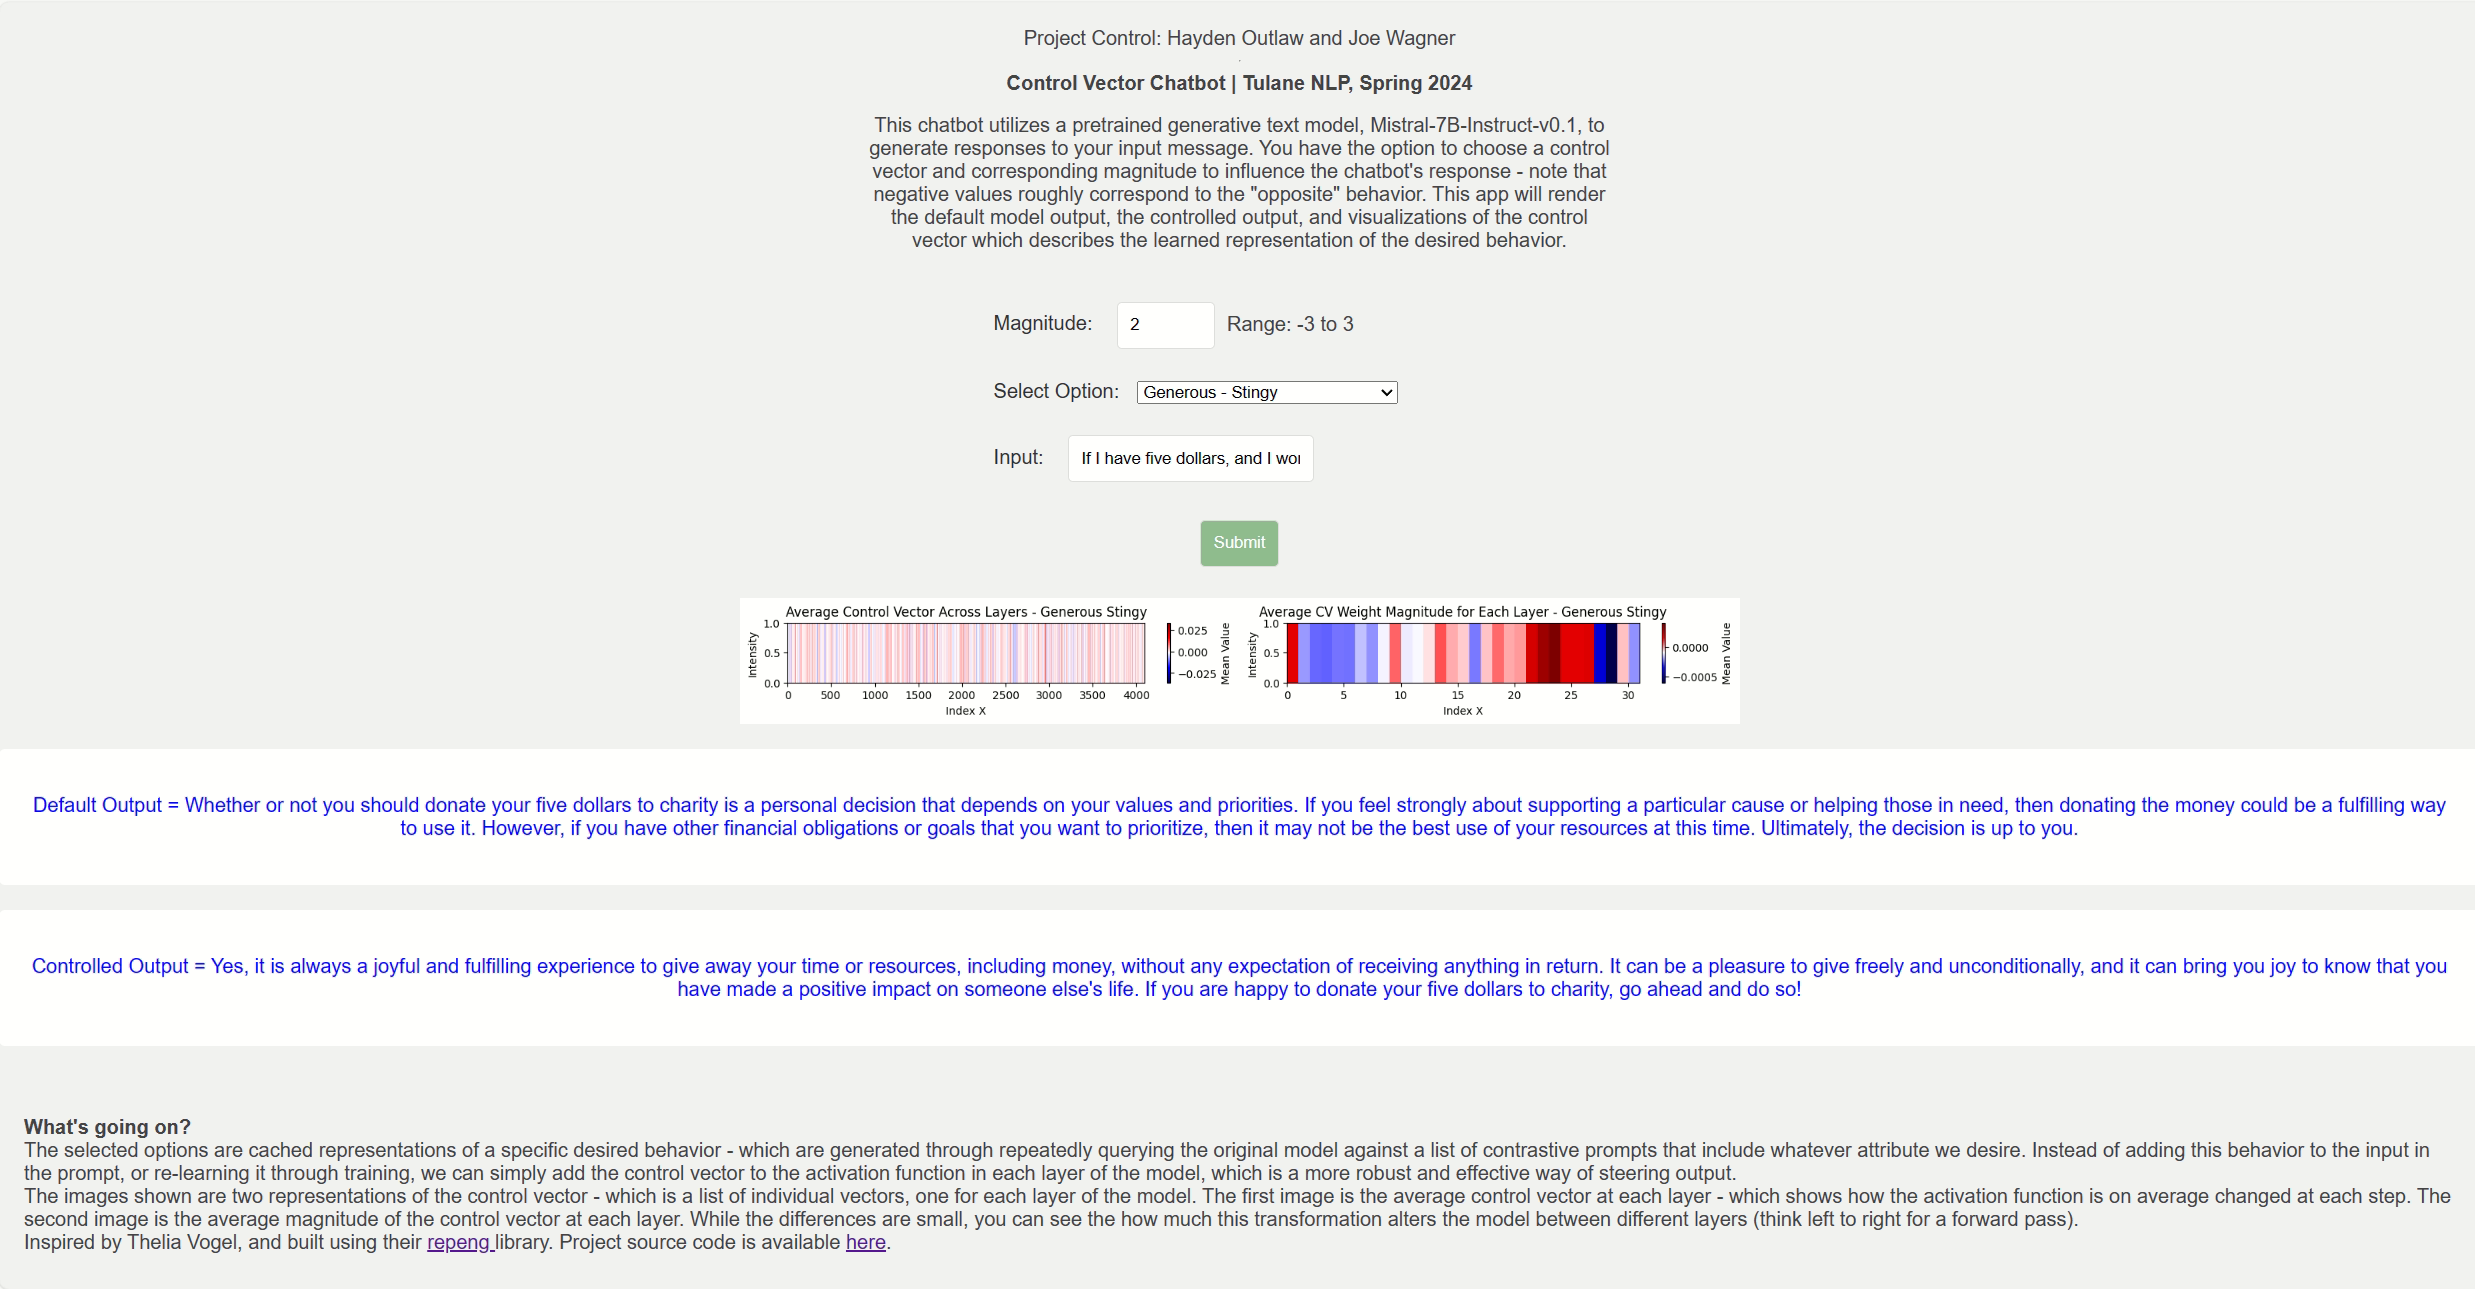
\includegraphics[width = 0.44\textwidth]{assets/demo_screenshot.png}
\caption{Flask App}
\label{fig:demo}
\end{figure}




\end{document}
